\documentclass[conference,letterpaper]{IEEEtran}
\usepackage[T1]{fontenc}
\usepackage[utf8]{inputenc}
\usepackage[spanish,es-tabla]{babel}
\usepackage{amsmath,amssymb}
\usepackage{graphicx,booktabs,url,array}
\usepackage{microtype}
\usepackage[hidelinks]{hyperref}
\hyphenation{LightGBM XGBoost CatBoost TransactionAmt TransactionDT}
\newcommand{\Ca}{C_a}
\newcommand{\ind}{\mathbf{1}}
\begin{document}
\renewcommand{\thesubsection}{\Alph{subsection}}
\renewcommand{\IEEEkeywordsname}{Palabras clave}
\title{Optimización basada en costos del umbral de decisión para el bloqueo de transacciones sospechosas mediante modelos de aprendizaje automático}
\author{\IEEEauthorblockN{Milton Alejandro Cuervo Ramírez, Oswald David Gutiérrez Cortina\\
y Diego Alejandro Rendón Suaza}
\IEEEauthorblockA{Departamento de Ingeniería de Sistemas, Facultad de Ingeniería\\
Universidad de Antioquia, Medellín, Colombia\\
\{milton.cuervo, oswaldd.gutierrez, diego.rendons\}@udea.edu.co}}
\maketitle

\begin{abstract}
El costo de aprobar una transacción fraudulenta depende de su monto, mientras que bloquearla y revisarla supone un gasto administrativo que también afecta a las compras legítimas. Esta diferencia motivó una comparación entre el corte fijo 0,5, Bayes Minimum Risk (BMR) y un árbol ponderado por costos sobre IEEE-CIS Fraud Detection. El experimento empleó 432 atributos y seleccionó LightGBM entre ocho configuraciones mediante dos ventanas temporales internas de entrenamiento. Su calibrador Platt se ajustó en validación temprana y las políticas se evaluaron, sin reajuste, en 84.233 operaciones posteriores con 2.960 fraudes. BMR obtuvo el menor costo global en los seis escenarios administrativos hipotéticos. Con un costo de revisión de 10 USD, redujo el costo 50,16\% frente al corte fijo y capturó 77,79\% del monto fraudulento, interviniendo 7,91\% de las legítimas. La mejora económica se explica por el equilibrio entre pérdidas evitadas y revisiones adicionales, aunque la calidad probabilística de Platt no mantuvo en prueba la mejora observada en validación. Los hallazgos respaldan una decisión dependiente del monto bajo la matriz adoptada; su alcance está condicionado por la intervención ideal, los costos administrativos hipotéticos y la consulta histórica de etiquetas agregadas del periodo final.
\end{abstract}
\begin{IEEEkeywords}
detección de fraude, costos dependientes del ejemplo, Bayes Minimum Risk, calibración probabilística, evaluación temporal.
\end{IEEEkeywords}

\section{Introducción}
La prevención del fraude exige decidir qué operaciones conviene intervenir sin someter todas las compras a revisión. Aprobar una operación fraudulenta puede comprometer su monto completo, pero bloquear una compra legítima también consume recursos y afecta al cliente. En consecuencia, una política que comete menos errores no necesariamente incurre en un costo menor, especialmente cuando transacciones con la misma etiqueta presentan montos muy distintos.

La distinción entre estimar la clase y elegir una acción tiene fundamento en la teoría de decisión sensible al costo de Elkan \cite{elkan}: bajo probabilidades verdaderas y errores simétricos, el corte 0,5 minimiza el error esperado de clasificación, mientras que una matriz asimétrica conduce a otra regla de acción. En fraude con tarjetas, Bahnsen et al. incorporaron el monto mediante BMR \cite{bmr} y estudiaron después la calidad de las probabilidades utilizadas para calcular riesgos \cite{calibrated}. Sus árboles dependientes del ejemplo modifican la partición y la poda \cite{csdt}, a diferencia de una aproximación basada en ponderar errores durante un ajuste convencional.

Almhaithawi et al. combinaron clasificación, remuestreo y BMR \cite{almhaithawi}, lo que sitúa el ahorro monetario como criterio de comparación más cercano al problema operativo que la exactitud global. Sin embargo, el uso económico de probabilidades también requiere comprobar su comportamiento futuro; por esa razón, la evaluación cronológica se apoya en el planteamiento de Dal Pozzolo et al. sobre poblaciones cambiantes y disponibilidad de etiquetas \cite{dalpozzolo}.

El objetivo general de este proyecto fue determinar en qué medida una regla dependiente del monto mejora el ahorro frente a una decisión convencional en IEEE-CIS. Los objetivos específicos consistieron en formalizar la matriz y su condición de intervención; establecer una referencia predictiva y probabilística con validación temporal y calibración; comparar el corte fijo, BMR y un árbol sensible al costo en condiciones comunes; y analizar la sensibilidad del ahorro ante variaciones del costo administrativo, incluidos posibles cambios de la estrategia con mejor desempeño. La pregunta que articula esos objetivos es si el riesgo económico individual permite obtener una decisión más conveniente que actuar únicamente según la etiqueta del clasificador.

El trabajo desarrolla una comparación experimental sobre datos públicos, con separación entre preparación, selección del predictor y evaluación de políticas. El corte clasificatorio se conserva en 0,5, de modo que el efecto económico se estudia en la etapa de decisión; la comparación no pretende introducir un algoritmo nuevo ni estimar los gastos operativos de una entidad particular.

\section{Metodología}
\subsection{Datos y preparación de las variables}
IEEE-CIS Fraud Detection contiene transacciones provistas por Vesta y publicadas en Kaggle \cite{dataset}. El archivo de operaciones etiquetadas reúne 590.540 filas y 394 columnas; la tabla de identidad aporta 144.233 filas y 41 columnas, incluida la clave compartida. La unión izquierda uno a uno por TransactionID conserva todas las operaciones y produce 434 columnas. La cobertura de identidad es 24,42\%, por lo que una unión interna restringiría el análisis a una población distinta de la que debe enfrentar el sistema.

Los 20.663 fraudes representan 3,499\% de las operaciones, y el 1\% de fraudes de mayor monto concentra 10,63\% del monto fraudulento. Este contraste entre frecuencia y exposición económica justifica evaluar tanto detección como pérdida residual. Además, 414 columnas presentan ausencias y 12 superan 90\%, con faltantes originados en las tablas y en la cobertura parcial de identidad. Las familias anonimizadas C, D, V e id se describen conforme a la información disponible, sin atribuir a cada variable un significado no publicado.

El monto TransactionAmt está expresado en dólares estadounidenses (USD), según la aclaración de la organización de la competencia sobre su conversión monetaria \cite{currency}. Los montos originales se conservan para evaluar costos; esa unidad documentada no convierte automáticamente el monto de una compra en una pérdida bancaria neta ni permite inferir el costo real de revisión.

La representación predictiva excluye identificador, tiempo crudo y etiqueta, y añade a los 431 atributos originales permitidos el indicador has\_identity, obtenido de la correspondencia de la unión. Las 432 entradas resultantes se distribuyen en 37 categóricas y 395 numéricas. Las categóricas incluyen producto, códigos de tarjeta y dirección, dominios de correo, M1--M9, dispositivo y quince columnas id de texto; sus vocabularios ordinales se aprenden solo en el pasado de ajuste. Las ausencias usan un token explícito y los niveles nuevos reciben $-1$, sin que los códigos representen distancia, magnitud o tasa de fraude.

Las numéricas se imputan con medianas aprendidas en el mismo pasado, tras convertir infinitos en ausencias; una columna completamente vacía se conserva con cero y advertencia. El preprocesador produce una matriz densa float32, mientras que el monto económico permanece aparte en float64. No se aplican remuestreo, pesos de clase, selección automática de columnas ni agregados históricos. Los clasificadores reciben las mismas entradas, aunque logística incorpora escalado sin centrar y CatBoost se evalúa sobre códigos numéricos, sin categorías nativas. Se conservan documentadas doce discrepancias de códigos id tratados numéricamente: 13, 14, 17--22, 24--26 y 32.

\subsection{Partición temporal y selección interna}
TransactionDT expresa segundos relativos sin origen calendario público y abarca aproximadamente 182 días. Los límites al 60\% y 80\% de la duración, seguidos por gaps de siete días, definen la Tabla~\ref{tab:split}; por ello, las fracciones de tiempo no equivalen a porcentajes de filas. Los gaps excluyen 41.399 operaciones del ajuste y la evaluación, y la validación se divide en mitades cronológicas manteniendo juntos los instantes simultáneos: la temprana ajusta Platt y la posterior diagnostica probabilidades y políticas. La prueba supervisada procede del conjunto etiquetado, ya que el test de Kaggle no publica etiquetas.

\begin{table}[t]
\caption{Distribución de los bloques temporales}
\label{tab:split}\centering\small
\begin{tabular}{lrr}\toprule
Bloque & Operaciones & Fraudes\\\midrule
Entrenamiento & 380\,815 & 13\,011\\
Gap 1: siete días & 20\,995 & 1\,015\\
Validación temprana & 42\,046 & 1\,558\\
Validación posterior & 42\,047 & 1\,517\\
Gap 2: siete días & 20\,404 & 602\\
Prueba final & 84\,233 & 2\,960\\\bottomrule
\end{tabular}
\end{table}

La selección compara XGBoost \cite{xgb}, LightGBM \cite{lgb}, CatBoost \cite{cat} y regresión logística con dos configuraciones acopladas por algoritmo. En la primera ventana interna se aprende hasta el 50\% de la duración de train y se evalúa después del gap hasta el 75\%; en la segunda se aprende hasta el 75\% y se evalúa después del gap hasta el final. Cada pasado ajusta sus propios vocabularios, medianas y escalador; los futuros contienen 62.815 y 68.759 operaciones. El segundo pasado incluye el primer futuro evaluado, como corresponde a una ventana expansiva, sin convertir las dos evaluaciones en réplicas independientes.

La Tabla~\ref{tab:config} presenta las configuraciones realmente ejecutadas. La búsqueda comprende ocho candidatos y dieciséis ajustes, no todas las combinaciones cartesianas de sus parámetros. La selección utiliza la media de Average Precision (AP) con igual peso por ventana y desempate lexicográfico exacto; no intervienen calibración, parada temprana ni costos posteriores en ese ranking. Esta selección estuvo precedida por una comparación exploratoria de las cuatro referencias en validación posterior, circunstancia que se conserva en la interpretación del diseño.

\begin{table*}[t]
\caption{Configuraciones evaluadas y parámetros de ajuste}
\label{tab:config}\centering\footnotesize
\renewcommand{\arraystretch}{1.12}
\begin{tabular}{>{\raggedright\arraybackslash}p{.11\textwidth}>{\raggedright\arraybackslash}p{.35\textwidth}>{\raggedright\arraybackslash}p{.22\textwidth}>{\raggedright\arraybackslash}p{.22\textwidth}}\toprule
Modelo & Parámetros fijos & Referencia & Regularizada\\\midrule
Boosting: común & 250 iteraciones; tasa 0,05; semilla 42; cuatro hilos & \multicolumn{2}{p{.45\textwidth}}{Dos configuraciones por algoritmo; mismo número de iteraciones y tasa.}\\
XGBoost & \texttt{subsample}=0,8; \texttt{colsample\_bytree}=0,8; método hist; objetivo \texttt{binary:logistic}; \texttt{eval\_metric}=aucpr & Profundidad 6; \texttt{min\_child\_weight}=10; L2 predeterminada & Profundidad 4; \texttt{min\_child\_weight}=20; \texttt{reg\_lambda}=10\\
LightGBM & \texttt{subsample}=0,8; \texttt{colsample\_bytree}=0,8; \texttt{subsample\_freq}=0 (predeterminado) & 63 hojas; mínimo 50 muestras por hoja; L2 predeterminada & 31 hojas; mínimo 100 muestras por hoja; \texttt{reg\_lambda}=5\\
CatBoost & \texttt{eval\_metric}=AUC; escritura automática desactivada; entrada ordinal numérica & Profundidad 6; L2 de hoja predeterminada & Profundidad 4; \texttt{l2\_leaf\_reg}=10\\
Logística & \texttt{solver}=saga; máximo 500 iteraciones; semilla 42; \texttt{StandardScaler(with\_mean=False)} & $C=0,1$ & $C=0,01$\\\midrule
Platt & Logit con recorte $10^{-6}$; \texttt{solver}=lbfgs; $C=10^6$; máximo 1.000 iteraciones & \multicolumn{2}{p{.45\textwidth}}{Un calibrador propio por predictor, ajustado en validación temprana.}\\
Árbol de acción & Profundidad 12; mínimo 250 muestras por hoja; semilla 42; impureza Gini; pesos por diferencia de costo & \multicolumn{2}{p{.45\textwidth}}{Un árbol por cada $\Ca\in\{1,5,10,20,50,100\}$ USD.}\\\bottomrule
\end{tabular}
\par\vspace{2pt}\begin{minipage}{.96\textwidth}\footnotesize
Los valores predeterminados son los de las versiones registradas: XGBoost 3.2.0, LightGBM 4.7.0, CatBoost 1.2.10 y scikit-learn 1.9.1. Las alternativas modifican parámetros de forma conjunta; no son ablaciones de un parámetro. En LightGBM, \texttt{subsample\_freq}=0 mantiene desactivado el muestreo de filas. Las métricas configuradas por biblioteca no reemplazan la AP común utilizada para seleccionar.
\end{minipage}
\end{table*}

\subsection{Matriz de costos y condición de intervención}
La etiqueta observada se denota $y_i\in\{0,1\}$, el monto original $A_i\geq0$ y el costo administrativo $\Ca>0$, ambos en USD. La matriz de la Tabla~\ref{tab:matrix} supone que bloquear y revisar evita toda la pérdida fraudulenta, con el mismo gasto en ambas clases; aprobar una legítima no incurre en costo dentro de este modelo.

\begin{table}[t]
\caption{Matriz de costos por transacción en USD}
\label{tab:matrix}\centering
\begin{tabular}{lcc}\toprule
Estado observado & Aprobar & Intervenir\\\midrule
Fraude & $A_i$ & $\Ca$\\
Legítima & $0$ & $\Ca$\\\bottomrule
\end{tabular}
\end{table}

Para una probabilidad estimada $p_i$, los riesgos esperados que compara BMR son
\begin{equation}
R_i(\text{aprobar})=p_iA_i,\qquad R_i(\text{intervenir})=\Ca.
\end{equation}
La intervención se activa si $p_iA_i>\Ca$, equivalente a $p_i>p_i^*=\Ca/A_i$ cuando $A_i>0$. La aprobación en empate y para $A_i=0$ evita decisiones sin ganancia estricta; cuando $A_i\leq\Ca$, ninguna probabilidad válida justifica intervenir bajo la matriz. La frontera es económica y dependiente de la operación, mientras que el corte clasificatorio permanece en 0,5.

El costo realizado de una política $d_i\in\{0,1\}$ es
\begin{equation}
C(d;\Ca)=\Ca\sum_i d_i+\sum_i y_iA_i(1-d_i).
\end{equation}
El ahorro trivial $S_{\rm ref}$ y la mejora frente a fija $M_{\rm fija}$ se calculan como
\begin{equation}
S_{\rm ref}=1-\frac{C(d;\Ca)}{C_{\rm ref}},\qquad M_{\rm fija}=1-\frac{C(d;\Ca)}{C_{\rm fija}},
\end{equation}
con $C_{\rm ref}=\min(\sum_i y_iA_i,N\Ca)$. Los denominadores distinguen la utilidad frente a una política aprendida de la utilidad frente a la mejor acción trivial, admitiendo valores negativos cuando una política resulta más costosa que su referencia.

\subsection{Calibración y políticas comparadas}
Antes de la selección interna, cada clasificador de referencia se entrenó con todo train y recibió su propio Platt, aprendido con las 42.046 operaciones tempranas. La transformación sigmoidal sobre logits \cite{niculescu} utiliza las probabilidades raw recortadas, sin acceder directamente a las 432 entradas:
\begin{equation}
\begin{aligned}
\widetilde p_i&=\min(1-\epsilon,\max(\epsilon,p_i^{\rm raw})),\\
p_i^{\rm cal}&=\sigma\left(a\log\frac{\widetilde p_i}{1-\widetilde p_i}+b\right),\quad\epsilon=10^{-6}.
\end{aligned}
\end{equation}
La selección de LightGBM coincidió con una referencia ya entrenada, lo que permitió verificar y reutilizar ese ajuste y su calibrador sin transferir parámetros desde otro modelo ni repetir entrenamientos idénticos. El análisis económico principal continuó con ese predictor; no se eligió entre los cuatro algoritmos por costo realizado.

La política fija interviene si $p_i^{\rm cal}\geq0,5$ y BMR aplica la condición de riesgo anterior. Como tercera política, un árbol por escenario aprende el objetivo $t_i=\ind[y_iA_i>\Ca]$ con peso $w_i=|y_iA_i-\Ca|$, normalizado por su media. El costo empírico se descompone en una constante más el error ponderado respecto a $t_i$, aunque el ajuste voraz por impureza no garantiza el mínimo global. El árbol recibe atributos y devuelve acciones; sus pesos representan diferencias económicas, no balanceo de clases, y no utiliza probabilidades de LightGBM.

Los escenarios administrativos son $\Ca\in\{1,5,10,20,50,100\}$ USD. Los valores pequeños se apoyan en antecedentes que estudian costos en euros de otras procesadoras \cite{bmr,calibrated}, tomados como orientación numérica y no como conversión o estimación para IEEE-CIS. Los seis valores permanecieron hipotéticos y fijados antes de test; 10 USD se emplea como ejemplo de lectura, sin seleccionarlo por el ahorro observado.

\subsection{Métricas y diagnóstico de resultados}
La AP común se calcula como suma de precisión ponderada por aumentos de recall, distinta de integrar la curva precisión--recall mediante trapecios. Brier y log-loss evalúan la calidad probabilística, mientras que recall, precisión y la tasa de falsas intervenciones $\mathrm{FPR}=FP/(FP+TN)$ describen las acciones al corte indicado. El recall por monto, $\sum_{i:y_i=1}A_id_i/\sum_{i:y_i=1}A_i$, permite establecer si la detección se concentra en pérdidas de mayor cuantía, sin confundirla con ahorro neto de revisión.

La validación posterior incluyó tres subperiodos y seis bandas de monto, así como concentración de fraude aprobado y sensibilidad de probabilidades. Después se fijaron modelo, calibrador, políticas, escenarios y métricas antes de test. Los subgrupos finales no ajustan decisiones; el boxplot describe las probabilidades individuales ya guardadas mediante cuartiles y bigotes de 1,5 rangos intercuartílicos, con media y frecuencia observada por banda. No representa intervalos de confianza ni genera nuevas predicciones.

La trazabilidad del repositorio \cite{repo} enlaza fuentes, manifiesto y resultados. Antes de test se verificó equivalencia entre entornos mediante doce tablas y tolerancias $10^{-8}$; la recuperación posterior consulta evidencia verificada sin repetir inferencia.

\section{Resultados y discusión}
\subsection{Comparación de modelos y confiabilidad probabilística}
La Tabla~\ref{tab:models} reúne las seis métricas de los ocho candidatos en las ventanas internas. LightGBM referencia alcanzó la mayor AP media, pero CatBoost referencia produjo alertas algo más precisas y una FPR menor al corte 0,5, junto con menor recall. Esa combinación explica por qué ``mejor clasificador'' depende del criterio: seleccionar precisión favorecería alertas más concentradas, mientras que AP prioriza el ordenamiento a través de umbrales. La elección de LightGBM resulta coherente con la regla declarada, sin demostrar que minimice el costo entre los cuatro algoritmos.

\begin{table*}[t]
\caption{Métricas predictivas de los modelos en validación temporal interna}
\label{tab:models}\centering\small
\begin{tabular}{lrrrrrr}\toprule
Configuración & AP & Brier & Log-loss & Recall (\%) & Precisión (\%) & FPR (\%)\\\midrule
LightGBM referencia & 0,58812 & 0,02329 & 0,09593 & 34,32 & 87,25 & 0,20 \\
LightGBM regularizada & 0,56857 & 0,02369 & 0,09772 & 33,63 & 87,48 & 0,19 \\
XGBoost referencia & 0,55486 & 0,02403 & 0,09953 & 32,28 & 87,42 & 0,19 \\
XGBoost regularizada & 0,52203 & 0,02514 & 0,10415 & 28,48 & 87,06 & 0,17 \\
CatBoost referencia & 0,51511 & 0,02526 & 0,10597 & 29,07 & 88,59 & 0,15 \\
CatBoost regularizada & 0,49123 & 0,02609 & 0,10920 & 26,85 & 87,40 & 0,16 \\
Logística referencia & 0,37069 & 0,02973 & 0,12467 & 16,44 & 82,62 & 0,14 \\
Logística regularizada & 0,37068 & 0,02973 & 0,12467 & 16,44 & 82,62 & 0,14 \\
\bottomrule\end{tabular}
\par\vspace{2pt}\begin{minipage}{.95\textwidth}\footnotesize
Métricas de probabilidades sin calibrar (raw), promediadas con igual peso por ventana. Recall, precisión y FPR usan corte 0,5; no son tasas de una matriz de confusión combinada. AP es el único criterio de selección. Menor Brier/log-loss es favorable; la FPR se interpreta junto con recall y costo de revisión.
\end{minipage}
\end{table*}

Las alternativas regularizadas no mejoraron AP respecto a sus referencias y las dos variantes logísticas quedaron prácticamente empatadas, por lo que la búsqueda realizada no aportó evidencia favorable a esas modificaciones conjuntas. La diferencia entre logística y boosting está condicionada por las entradas ordinales: un efecto lineal sobre códigos arbitrarios es más restrictivo que separar sus rangos mediante árboles. La comparación no permite atribuir la brecha únicamente al algoritmo ni descartar otra representación para logística o categorías nativas en CatBoost.

La Tabla~\ref{tab:prob} muestra que la mejora de Brier y log-loss con Platt en validación posterior no se trasladó a test. En cambio, AP se mantuvo entre raw y Platt dentro de cada población porque la transformación conservó el orden de riesgo en esta corrida. El contraste indica que ordenar transacciones y asignarles probabilidades adecuadas son propiedades diferentes: la media Platt pasó de quedar por debajo de la prevalencia de validación (3,61\%) a quedar por encima de la de test (3,51\%). Se mantuvo el calibrador previamente fijado, evitando seleccionarlo con la población final.

\begin{table}[t]
\caption{Calidad probabilística de LightGBM en validación y prueba}
\label{tab:prob}\centering\small
\begin{tabular}{llrrr}\toprule
Población & Probabilidad & AP & Brier & Log-loss\\\midrule
Validación & Raw & 0,50440 & 0,02435 & 0,09750\\
posterior & Platt & 0,50440 & 0,02406 & 0,09645\\
Prueba & Raw & 0,51780 & 0,02279 & 0,09471\\
final & Platt & 0,51780 & 0,02300 & 0,09515\\\bottomrule
\end{tabular}
\end{table}

\subsection{Costo y compromiso de intervención}
La Tabla~\ref{tab:costs} evidencia una ventaja global de BMR en los seis costos administrativos. Esa ventaja no debe leerse como una reducción uniforme ni como prueba de optimalidad para cualquier costo: al aumentar $\Ca$, intervenir requiere un riesgo esperado mayor y cambia qué operaciones compensan el gasto de revisión. También cambia la referencia trivial, de intervenir todo con 1 y 5 USD a aprobar todo desde 10 USD en la cuadrícula evaluada.

\begin{table}[t]
\caption{Costo total de las políticas por escenario administrativo en USD}
\label{tab:costs}\centering\small
\begin{tabular}{rrrr}\toprule
$\Ca$ (USD) & Fija 0,5 & BMR & Árbol\\\midrule
1 & 350\,614,63 & \textbf{50\,285,76} & 86\,169,78 \\
5 & 356\,326,63 & \textbf{126\,957,37} & 167\,704,70 \\
10 & 363\,466,63 & \textbf{181\,140,26} & 228\,707,97 \\
20 & 377\,746,63 & \textbf{226\,249,60} & 276\,727,44 \\
50 & 420\,586,63 & \textbf{309\,995,57} & 357\,072,31 \\
100 & 491\,986,63 & \textbf{374\,372,19} & 400\,085,92 \\
\bottomrule\end{tabular}
\end{table}

Con $\Ca=10$ USD, BMR redujo el costo 50,16\% frente a fija y 59,91\% frente a aprobar todo, que es la mejor referencia trivial del escenario. La explicación aparece al separar componentes: frente a fija se añadieron 66.530 USD de gasto de intervención y se redujo en 248.856,371 USD el monto de fraude aprobado, para una reducción neta de 182.326,371 USD. El beneficio provino, por tanto, de evitar suficiente exposición económica para compensar revisiones adicionales, no de eliminar falsos positivos.

La Tabla~\ref{tab:operation} permite interpretar ese intercambio. La precisión de BMR fue menor porque una fracción más alta de sus intervenciones correspondió a legítimas, pero su captura monetaria aumentó mucho más que el recall por cantidad. La Figura~\ref{fig:tradeoff}, titulada ``Compromiso entre intervención de legítimas y captura monetaria'', muestra que las políticas se desplazan por combinaciones operativas distintas: una entidad con capacidad limitada de revisión no podría adoptar estos resultados sin incorporar esa restricción.

\begin{table}[t]
\caption{Indicadores operativos de las políticas con costo administrativo de 10 USD}
\label{tab:operation}\centering\small
\begin{tabular}{lrrrr}\toprule
Política & Alertas & Recall & FPR & Recall monto\\\midrule
Fija 0,5 & 1\,428 & 37,26\% & 0,40\% & 22,71\%\\
BMR & 8\,081 & 55,84\% & 7,91\% & 77,79\%\\
Árbol & 7\,212 & 42,43\% & 7,33\% & 65,34\%\\\bottomrule
\end{tabular}
\end{table}

\begin{figure}[t]
\centering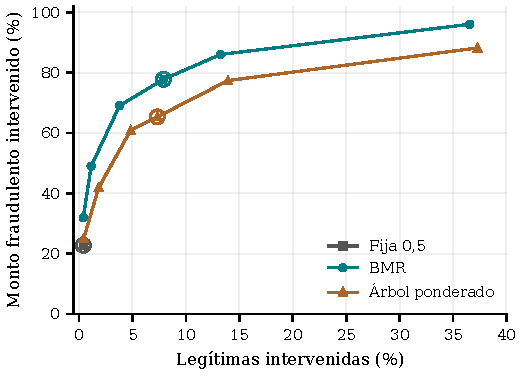
\includegraphics[width=\columnwidth]{compromiso_operativo.pdf}
\caption{Compromiso entre intervención de legítimas y captura monetaria. Cada punto corresponde a un escenario; los círculos abiertos indican $\Ca=10$ USD. Fija ocupa un punto porque sus acciones no dependen de $\Ca$. Las líneas solo conectan los seis escenarios evaluados.}
\label{fig:tradeoff}
\end{figure}

La comparación con referencias triviales evita una conclusión engañosa cuando una política mejora frente a fija, pero sigue siendo innecesariamente costosa. Con $\Ca=1$ USD, el árbol supera el costo de intervenir todas las operaciones; con $\Ca=100$ USD, fija supera el costo de aprobar todo. La permanencia del mismo corte conserva acciones entre escenarios, aunque la conveniencia económica de esas acciones cambia con el precio de revisión.

\subsection{Sensibilidad temporal y heterogeneidad por monto}
La ventaja agregada no describió todos los subperiodos de desarrollo: BMR tuvo el menor costo en 17 de 18 combinaciones periodo/$\Ca$ de validación, con una excepción favorable al árbol en el tercer periodo y 100 USD. En test ganó las 18 combinaciones, pero su FPR con 10 USD aumentó de 5,78\% en validación a 7,91\%, mientras la mejora frente a fija bajó de 57,51\% a 50,16\%. Esto sugiere que conservar una ventaja relativa no equivale a conservar la carga de revisión, una diferencia relevante para trasladar la política a periodos futuros.

La Figura~\ref{fig:bands}, ``Distribución de probabilidades Platt por monto'', permite observar que operaciones de un mismo rango monetario reciben riesgos heterogéneos. En [500,1000) USD la mediana de probabilidad es 1,79\% y la media 5,84\%, lo que evidencia una cola de riesgos altos dentro de la banda; sustituir esas probabilidades por un único promedio eliminaría información que interviene en la decisión individual. La frecuencia observada de 7,38\% supera la media estimada y mantiene la subestimación detectada en validación, aunque el boxplot por sí solo no constituye una prueba de calibración: la caja resume probabilidades individuales, no la incertidumbre de esa frecuencia.

\begin{figure}[t]
\centering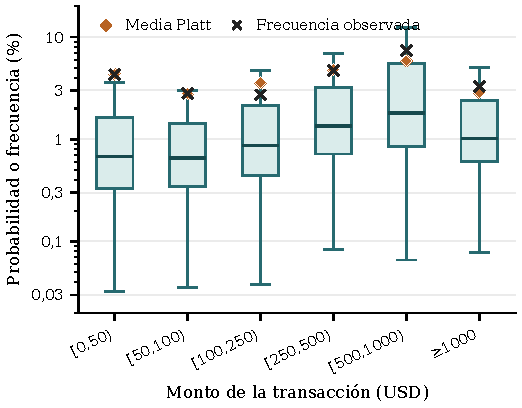
\includegraphics[width=\columnwidth]{calibracion_por_monto.pdf}
\caption{Distribución de probabilidades Platt por monto. Cajas entre cuartiles 1 y 3, línea mediana y bigotes a las observaciones extremas dentro de 1,5 rangos intercuartílicos; se omiten los puntos externos. Los diamantes indican la media y las cruces la frecuencia observada. El eje vertical es logarítmico y las bandas de monto están en USD.}
\label{fig:bands}
\end{figure}

El desajuste monetario de [500,1000) equivale a 93.714,35 USD esperados frente a 128.656,95 USD de fraude observado, mientras que [100,250) presenta sobreestimación. La exposición global queda apenas 2,07\% por debajo de la observada porque diferencias de signos opuestos se compensan. Esa cercanía global no garantiza decisiones adecuadas en cada banda y explica por qué los diagnósticos de monto añaden información que no proporcionan AP o la probabilidad media.

La sensibilidad examinada no identificó un cambio de ganador global entre los seis costos administrativos. La excepción temporal de validación impide extender esa estabilidad a toda subpoblación, y la cuadrícula discreta no permite establecer rangos continuos de optimalidad. La evidencia responde al análisis de escenarios previsto, sin forzar la existencia de una transición que los datos no mostraron.

\clearpage
\section{Limitaciones}
La matriz supone intervención totalmente eficaz y excluye capacidad de revisión, recuperaciones y perjuicio comercial adicional; aunque los montos están en USD, los costos administrativos no fueron estimados para una entidad real. La selección por AP, la representación ordinal, los doce id numéricos y CatBoost sin categorías nativas también condicionan el alcance de la comparación, sin que se haya realizado una ablación que separe esos efectos.

La evaluación conserva orden cronológico, pero el EDA y la selección histórica de gaps consultaron etiquetas agregadas del periodo final; por ello, no constituye una reserva completamente ciega desde el diseño. La validación posterior se usó como desarrollo y los dos futuros internos no son réplicas independientes. Los subgrupos y el boxplot son diagnósticos descriptivos, sin intervalos de confianza ni pruebas de superioridad estadística. Las políticas finales permanecieron fijas después de consultar test; cualquier selección posterior requerirá otro experimento y una población nueva.

\section{Conclusiones}
La formalización de costos permitió establecer que el monto modifica la acción conveniente aun cuando la etiqueta del clasificador sea la misma. La condición $p_iA_i>\Ca$ ofrece una interpretación operativa del primer objetivo: intervenir depende de cuánto riesgo económico se evita y no solo de que una transacción supere un umbral de fraude. Cuando el monto no supera el costo administrativo, la propia matriz descarta una intervención con ganancia esperada estricta.

La referencia temporal mostró que discriminación y confiabilidad probabilística deben examinarse por separado. LightGBM fue la configuración seleccionada bajo el criterio declarado, pero Platt no conservó en prueba la mejora probabilística de validación. Este hallazgo limita el uso de una calibración como garantía permanente y refuerza la necesidad de revisar los grupos de monto, donde un promedio global cercano puede ocultar errores económicamente importantes.

La comparación de políticas respondió favorablemente al objetivo económico: incorporar riesgo y monto mediante BMR resultó más conveniente que actuar según la etiqueta en los escenarios estudiados. El mecanismo observado fue la compensación de revisiones adicionales con una menor exposición a fraude aprobado, de modo que una caída en precisión no implicó por sí misma una peor decisión. La utilidad demostrada en esta muestra corresponde a la matriz asumida y no sustituye la evaluación de capacidad o de efectos sobre clientes.

La sensibilidad no reveló una transición del ganador global dentro de los seis costos examinados, aunque sí variación temporal del beneficio y una excepción de desarrollo favorable al árbol. El cuarto objetivo queda respondido en términos de escenarios discretos: la permanencia de BMR como mejor alternativa global es un hallazgo, mientras que los rangos continuos de cambio de estrategia permanecen sin identificar. La continuidad requiere costos administrativos observados y otra evaluación temporal independiente.

\noindent\begin{minipage}{\columnwidth}
\section*{Agradecimientos}
Se agradece a la profesora María Bernarda Salazar Sánchez el acompañamiento y la revisión metodológica durante Proyecto Integrador II de Ingeniería de Sistemas, Universidad de Antioquia.
\end{minipage}

\begin{thebibliography}{13}
\bibitem{elkan} C. Elkan, ``The foundations of cost-sensitive learning,'' in \emph{Proc. IJCAI}, 2001, pp. 973--978.
\bibitem{bmr} A. C. Bahnsen, A. Stojanovic, D. Aouada, and B. Ottersten, ``Cost sensitive credit card fraud detection using Bayes minimum risk,'' in \emph{Proc. ICMLA}, vol. 1, 2013, pp. 333--338, doi: 10.1109/ICMLA.2013.68.
\bibitem{calibrated} A. C. Bahnsen, A. Stojanovic, D. Aouada, and B. Ottersten, ``Improving credit card fraud detection with calibrated probabilities,'' in \emph{Proc. SIAM SDM}, 2014, pp. 677--685, doi: 10.1137/1.9781611973440.78.
\bibitem{csdt} A. C. Bahnsen, D. Aouada, and B. Ottersten, ``Example-dependent cost-sensitive decision trees,'' \emph{Expert Syst. Appl.}, vol. 42, no. 19, pp. 6609--6619, 2015, doi: 10.1016/j.eswa.2015.04.042.
\bibitem{almhaithawi} D. Almhaithawi, A. Jafar, and M. Aljnidi, ``Example-dependent cost-sensitive credit cards fraud detection using SMOTE and Bayes minimum risk,'' \emph{SN Appl. Sci.}, vol. 2, art. 1574, 2020, doi: 10.1007/s42452-020-03375-w.
\bibitem{dalpozzolo} A. Dal Pozzolo, G. Boracchi, O. Caelen, C. Alippi, and G. Bontempi, ``Credit card fraud detection: A realistic modeling and a novel learning strategy,'' \emph{IEEE Trans. Neural Netw. Learn. Syst.}, vol. 29, no. 8, pp. 3784--3797, 2018, doi: 10.1109/TNNLS.2017.2736643.
\bibitem{dataset} IEEE Computational Intelligence Society and Vesta Corporation, ``IEEE-CIS Fraud Detection,'' Kaggle, 2019. [Online]. Available: \url{https://www.kaggle.com/competitions/ieee-fraud-detection/data}
\bibitem{currency} Vesta Corporation, ``IEEE-CIS Fraud Detection: respuestas de la organización sobre los datos,'' Kaggle, 2019. [En línea]. Disponible: \url{https://www.kaggle.com/competitions/ieee-fraud-detection/discussion/100304}. Consulta: 10 nov. 2026.
\bibitem{xgb} T. Chen and C. Guestrin, ``XGBoost: A scalable tree boosting system,'' in \emph{Proc. ACM SIGKDD}, 2016, pp. 785--794, doi: 10.1145/2939672.2939785.
\bibitem{lgb} G. Ke \emph{et al.}, ``LightGBM: A highly efficient gradient boosting decision tree,'' in \emph{Adv. Neural Inf. Process. Syst.}, vol. 30, 2017, pp. 3146--3154.
\bibitem{cat} L. Prokhorenkova, G. Gusev, A. Vorobev, A. V. Dorogush, and A. Gulin, ``CatBoost: Unbiased boosting with categorical features,'' in \emph{Adv. Neural Inf. Process. Syst.}, vol. 31, 2018, pp. 6638--6648.
\bibitem{niculescu} A. Niculescu-Mizil and R. Caruana, ``Predicting good probabilities with supervised learning,'' in \emph{Proc. ICML}, 2005, pp. 625--632, doi: 10.1145/1102351.1102430.
\bibitem{repo} M. A. Cuervo Ramírez, O. D. Gutiérrez Cortina, and D. A. Rendón Suaza, ``IEEE-CIS Fraud Detection--PI2: código y evidencia experimental,'' 2026. [Online]. Available: \url{https://github.com/MiltonCuervo/IEEE-CIS-Fraud-Detection-PI2}
\end{thebibliography}
\end{document}
